%% ========================================================
%% CHAPTER 5: SYSTEM DESIGN
%% ========================================================
\chapter{System Design}
\section{System Architecture}

The system operates as a three-tier edge pipeline: a camera source captures live video, an edge computing unit processes frames through a detection-OCR-verification pipeline, and an authorization signal is issued to the charging hardware. The architecture is designed for minimal latency and maximum autonomy.

\begin{figure}[H]
  \centering
  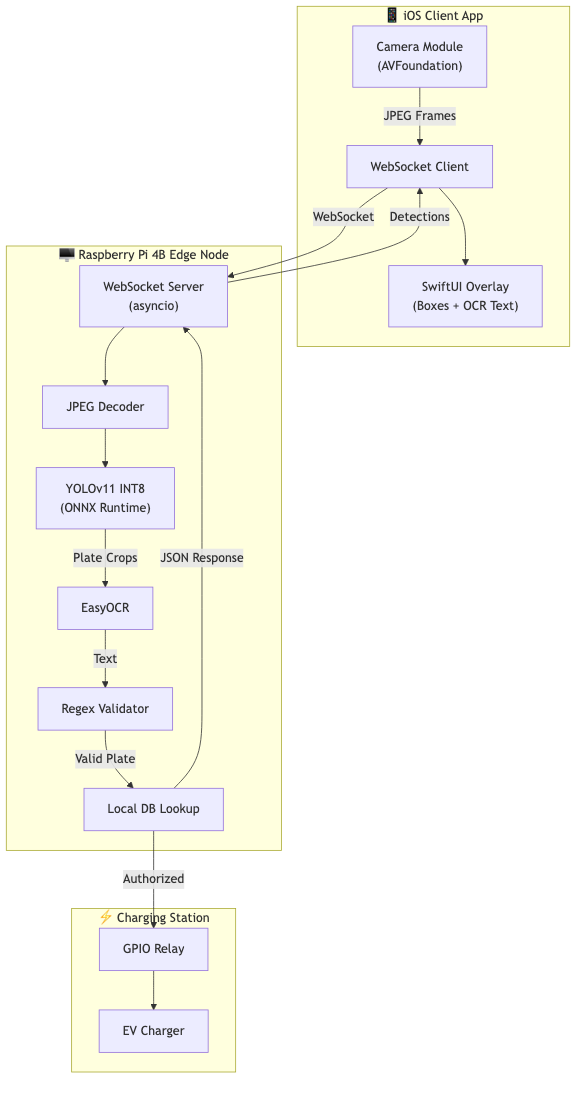
\includegraphics[width=4in]{architecture.png}
  \caption{System Architecture Diagram}
  \label{fig:arch}
\end{figure}

\subsection{Architectural Design Principles}
The system design follows these key principles:
\begin{enumerate}
    \item \textbf{Edge-First Processing:} All inference and verification occurs locally on the Raspberry Pi. No data leaves the local network during normal operation.
    \item \textbf{Asynchronous Communication:} WebSocket-based bidirectional streaming enables real-time frame processing without polling overhead.
    \item \textbf{Modular Pipeline:} Each stage (detection, OCR, validation, lookup) is independently replaceable without affecting other stages.
    \item \textbf{Fail-Safe Design:} Unrecognized plates result in no action (detection overlay only), not false authorization.
\end{enumerate}

\section{Use Case Diagram}

\begin{figure}[H]
\centering
\begin{tikzpicture}[
    actor/.style={circle, draw, minimum size=0.8cm, font=\small},
    usecase/.style={ellipse, draw, fill=blue!8, text width=2.8cm, text centered, minimum height=0.8cm, font=\small},
    arrow/.style={->, thick}
]
\node[actor] (driver) at (0,0) {Driver};
\node[actor] (admin) at (0,-6) {Admin};
\node[usecase] (park) at (5, 1) {Park at Station};
\node[usecase] (detect) at (5, -0.5) {Plate Detected};
\node[usecase] (verify) at (5, -2) {Verify Identity};
\node[usecase] (charge) at (5, -3.5) {Begin Charging};
\node[usecase] (view) at (5, -5) {View Status};
\node[usecase] (manage) at (5, -6.5) {Manage Database};
\node[usecase] (update) at (5, -8) {Update Model};
\draw[arrow] (driver) -- (park);
\draw[arrow] (driver) -- (view);
\draw[arrow] (park) -- (detect);
\draw[arrow] (detect) -- (verify);
\draw[arrow] (verify) -- (charge);
\draw[arrow] (admin) -- (manage);
\draw[arrow] (admin) -- (update);
\end{tikzpicture}
\caption{Use Case Diagram}
\label{fig:usecase}
\end{figure}

\section{Data Flow Diagrams}
\subsection{Level 0 DFD (Context Diagram)}

\begin{figure}[H]
\centering
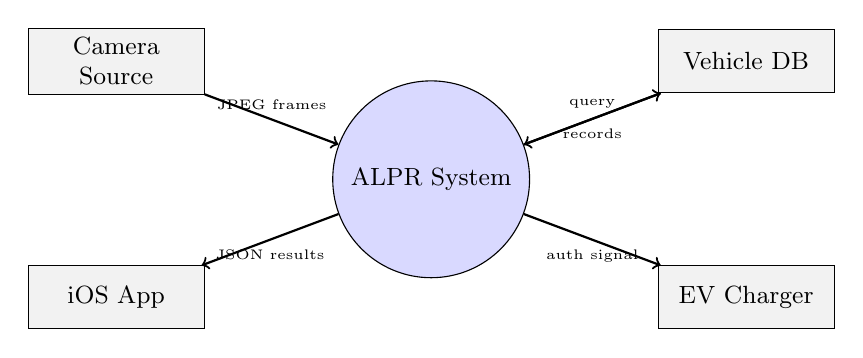
\begin{tikzpicture}[
    entity/.style={rectangle, draw, fill=gray!10, text width=2cm, text centered, minimum height=0.8cm, font=\small},
    process/.style={circle, draw, fill=blue!15, minimum size=2.5cm, text centered, font=\small},
    arrow/.style={->, thick}
]
\node[entity] (camera) at (-4, 1.5) {Camera Source};
\node[entity] (ios) at (-4, -1.5) {iOS App};
\node[process] (system) at (0, 0) {ALPR System};
\node[entity] (db) at (4, 1.5) {Vehicle DB};
\node[entity] (charger) at (4, -1.5) {EV Charger};
\draw[arrow] (camera) -- node[above, font=\tiny]{JPEG frames} (system);
\draw[arrow] (system) -- node[below, font=\tiny]{JSON results} (ios);
\draw[arrow] (system) -- node[above, font=\tiny]{query} (db);
\draw[arrow] (db) -- node[below, font=\tiny]{records} (system);
\draw[arrow] (system) -- node[below, font=\tiny]{auth signal} (charger);
\end{tikzpicture}
\caption{Level 0 Data Flow Diagram}
\label{fig:dfd0}
\end{figure}

\subsection{Level 1 DFD}

\begin{figure}[H]
\centering
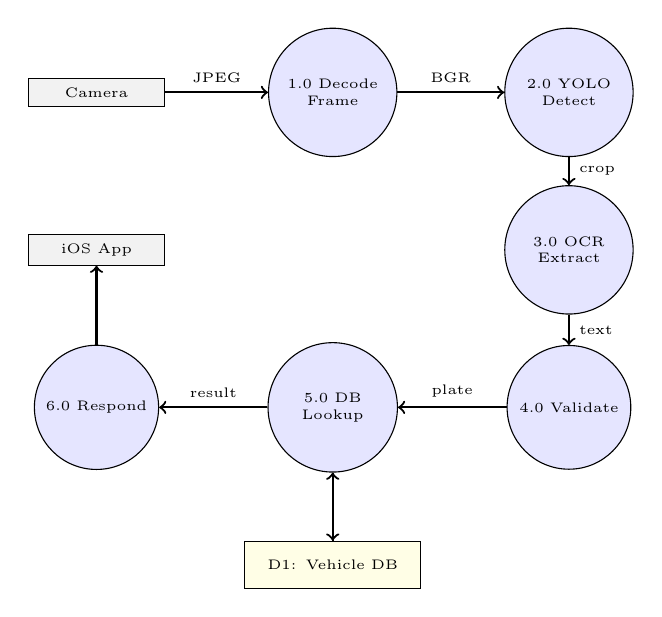
\begin{tikzpicture}[
    process/.style={circle, draw, fill=blue!10, minimum size=1.5cm, text centered, font=\tiny, text width=1.3cm},
    store/.style={rectangle, draw, fill=yellow!10, text width=2cm, text centered, minimum height=0.6cm, font=\tiny},
    entity/.style={rectangle, draw, fill=gray!10, text width=1.5cm, text centered, font=\tiny},
    arrow/.style={->, thick, font=\tiny}
]
\node[entity] (cam) at (-3, 2) {Camera};
\node[process] (decode) at (0, 2) {1.0 Decode Frame};
\node[process] (yolo) at (3, 2) {2.0 YOLO Detect};
\node[process] (ocr) at (3, 0) {3.0 OCR Extract};
\node[process] (validate) at (3, -2) {4.0 Validate};
\node[process] (lookup) at (0, -2) {5.0 DB Lookup};
\node[process] (respond) at (-3, -2) {6.0 Respond};
\node[store] (db) at (0, -4) {D1: Vehicle DB};
\node[entity] (ios) at (-3, 0) {iOS App};
\draw[arrow] (cam) -- node[above]{JPEG} (decode);
\draw[arrow] (decode) -- node[above]{BGR} (yolo);
\draw[arrow] (yolo) -- node[right]{crop} (ocr);
\draw[arrow] (ocr) -- node[right]{text} (validate);
\draw[arrow] (validate) -- node[above]{plate} (lookup);
\draw[arrow] (lookup) -- node[above]{result} (respond);
\draw[arrow] (lookup) -- (db);
\draw[arrow] (db) -- (lookup);
\draw[arrow] (respond) -- (ios);
\end{tikzpicture}
\caption{Level 1 Data Flow Diagram}
\label{fig:dfd1}
\end{figure}

\section{Database Design}

The system uses SQLite for persistent vehicle data storage. The schema is designed for simplicity and fast lookups.

\subsection{Entity-Relationship Diagram}
\begin{figure}[H]
\centering
\begin{tikzpicture}[
    entity/.style={rectangle, draw, fill=blue!10, text width=2.5cm, text centered, minimum height=1cm, font=\small},
    attr/.style={ellipse, draw, fill=green!10, text width=1.5cm, text centered, font=\tiny}
]
\node[entity] (vehicle) at (0, 0) {\textbf{Vehicle}};
\node[attr] (plate) at (-3, 1.5) {plate\_number (PK)};
\node[attr] (owner) at (0, 2) {owner\_name};
\node[attr] (balance) at (3, 1.5) {balance};
\node[attr] (reg) at (-3, -1.5) {reg\_date};
\node[attr] (status) at (3, -1.5) {status};
\draw (vehicle) -- (plate);
\draw (vehicle) -- (owner);
\draw (vehicle) -- (balance);
\draw (vehicle) -- (reg);
\draw (vehicle) -- (status);
\end{tikzpicture}
\caption{Entity-Relationship Diagram for Vehicle Database}
\label{fig:er}
\end{figure}

\subsection{Database Schema}
\begin{table}[H]
\centering
\caption{Vehicle Table Schema}
\renewcommand{\arraystretch}{1.3}
\begin{tabular}{|l|l|l|l|}
\hline
\textbf{Column} & \textbf{Type} & \textbf{Constraint} & \textbf{Description} \\
\hline
plate\_number & TEXT & PRIMARY KEY & License plate string \\
\hline
owner\_name & TEXT & NOT NULL & Registered owner's name \\
\hline
balance & REAL & DEFAULT 0.0 & Account balance (INR) \\
\hline
registration\_date & TEXT & DEFAULT CURRENT\_TIMESTAMP & Registration date \\
\hline
status & TEXT & DEFAULT `active' & Account status \\
\hline
\end{tabular}
\end{table}

\section{Module Description}

\subsection{Module 1: Camera Streaming Module (iOS)}
The Camera Streaming Module captures live video frames using AVFoundation's \texttt{AVCaptureSession}. It configures the rear camera at 1280$\times$720 resolution, captures individual frames via \texttt{AVCaptureVideoDataOutput}, compresses each frame to JPEG (quality 0.6), and transmits the binary data via WebSocket.

On the receiving side, the module listens for JSON responses from the server. When detections are received, it parses bounding box coordinates and OCR text, rendering them as colored rectangles on a transparent overlay view positioned above the camera preview. When a verification response is received, it stops the camera session and presents a modal view displaying the owner's name and balance.

\textbf{Key Components:}
\begin{itemize}
    \item \texttt{CameraManager}: Handles AVCaptureSession lifecycle.
    \item \texttt{WebSocketManager}: Manages connection, sending frames, receiving JSON.
    \item \texttt{DetectionOverlay}: SwiftUI view that renders bounding boxes.
    \item \texttt{VerificationModal}: Success screen with owner details.
\end{itemize}

\subsection{Module 2: Edge Inference Module (Raspberry Pi)}
The Edge Inference Module is the core processing unit. It receives JPEG frames via WebSocket, decodes them using OpenCV (\texttt{cv2.imdecode}), and prepares them for YOLO inference by resizing to 640$\times$640, normalizing pixel values to [0,1], and transposing to NCHW format.

The ONNX Runtime \texttt{InferenceSession} executes the quantized INT8 model, producing raw detection outputs. Post-processing includes sigmoid activation on objectness scores, bounding box coordinate decoding (center to corner format), confidence thresholding (0.25), and Non-Maximum Suppression (IoU threshold 0.45).

\textbf{Key Components:}
\begin{itemize}
    \item \texttt{InferenceSession}: ONNX Runtime session for INT8 model.
    \item \texttt{preprocess()}: Image resize, normalize, transpose.
    \item \texttt{postprocess()}: NMS, box decode, score filter.
    \item \texttt{handle\_connection()}: Async WebSocket connection handler.
\end{itemize}

\subsection{Module 3: OCR and Validation Module}
The OCR module processes cropped plate regions through EasyOCR. It uses a pre-trained English character recognition model (CRNN architecture) to extract text. The raw output is cleaned by:
\begin{enumerate}
    \item Removing all whitespace characters.
    \item Converting to uppercase.
    \item Stripping non-alphanumeric characters.
\end{enumerate}

The cleaned text is then validated against a regex pattern matching standard Indian license plate formats: \texttt{\^{}[A-Z]\{2\}[0-9]\{2\}[A-Z]\{1,2\}[0-9]\{4\}\$}

This pattern matches plates like KL07AB1234, MH12DE1433, DL01C0001, etc.

\subsection{Module 4: Database and Verification Module}
The Database Module manages vehicle records in SQLite. When a validated plate string is received, it executes:
\begin{verbatim}
SELECT owner_name, balance FROM vehicles 
WHERE plate_number = ? AND status = 'active'
\end{verbatim}

If a match is found, a JSON verification payload is generated:
\begin{verbatim}
{
  "type": "verification",
  "plate": "KL07AB1234",
  "owner": "Joel K George",
  "balance": "500.00",
  "verified": true
}
\end{verbatim}

%% ========================================================
%% CHAPTER 6: IMPLEMENTATION
%% ========================================================
\chapter{Implementation}
\section{Model Quantization Pipeline}

The quantization pipeline converts the YOLOv11 model from FP32 to INT8 precision. This section describes each step in detail.

\subsection{Step 1: ONNX Model Export}
The YOLOv11 model, trained on a license plate detection dataset, is first exported from PyTorch to ONNX format using the Ultralytics export API:
\begin{verbatim}
from ultralytics import YOLO
model = YOLO('best.pt')
model.export(format='onnx', imgsz=640, opset=17)
\end{verbatim}

This produces an FP32 ONNX model of approximately 200\,MB.

\subsection{Step 2: Calibration Data Preparation}
Static quantization requires a representative calibration dataset to determine the dynamic range of activations at each layer. We prepare 100 representative license plate images:
\begin{verbatim}
class CalibrationDataReader:
    def __init__(self, calibration_dir):
        self.images = glob(f"{calibration_dir}/*.jpg")
        self.index = 0
    
    def get_next(self):
        if self.index >= len(self.images):
            return None
        img = preprocess(self.images[self.index])
        self.index += 1
        return {'images': img}
\end{verbatim}

\subsection{Step 3: Static INT8 Quantization}
The ONNX model is quantized using ONNX Runtime's quantization tools:

\begin{algorithm}[H]
\caption{Static INT8 Quantization}
\begin{algorithmic}[1]
\Function{QuantizeModel}{$modelPath, calibrationDir$}
    \State $model \gets$ Load ONNX model from $modelPath$
    \State $reader \gets$ CalibrationDataReader($calibrationDir$)
    \State Configure: weight\_type $\gets$ INT8, activation\_type $\gets$ INT8
    \State Configure: per\_channel $\gets$ True, reduce\_range $\gets$ False
    \State $quantModel \gets$ StaticQuantize($model$, $reader$, config)
    \State Save $quantModel$ to ``quantized\_model.onnx''
    \State \Return $quantModel$
\EndFunction
\end{algorithmic}
\end{algorithm}

The resulting INT8 model is approximately 25\,MB---an 87.5\% reduction.

\subsection{Step 4: ONNX Graph Patching (INT8 to UINT8)}
A critical challenge emerged during deployment: the ONNX Runtime ARM CPU execution provider does not support signed INT8 weights in \texttt{ConvInteger} nodes. The error manifests as:
\begin{verbatim}
NOT_IMPLEMENTED: ConvInteger with signed weight 
is not supported on ARM CPU
\end{verbatim}

To resolve this without retraining, we developed a custom graph patching script that shifts all signed INT8 weights into the unsigned UINT8 domain:

\begin{algorithm}[H]
\caption{Fix INT8 to UINT8 Weights}
\begin{algorithmic}[1]
\Function{FixQuantization}{$modelPath, outputPath$}
    \State $model \gets$ Load ONNX model from $modelPath$
    \State $initializers \gets$ Map of initializers by name
    \For{each $node$ in $model.graph.node$}
        \If{$node.opType$ == ``ConvInteger''}
            \State $W \gets$ weight tensor from $initializers[node.input[1]]$
            \State $Z_w \gets$ zero-point from $initializers[node.input[3]]$
            \If{$W.dataType$ == INT8}
                \State $W_{uint8} \gets \text{cast}(W_{int8} + 128, \text{UINT8})$
                \State $Z_{w,uint8} \gets \text{cast}(Z_{w,int8} + 128, \text{UINT8})$
                \State Replace tensors in model graph
                \State Update data type to UINT8
            \EndIf
        \EndIf
    \EndFor
    \State $onnx.checker.check\_model(model)$
    \State Save model to $outputPath$
\EndFunction
\end{algorithmic}
\end{algorithm}

\subsection{Quantization Impact Analysis}

Figure~\ref{fig:model_size} shows the model size comparison, and Figure~\ref{fig:inference_speed} shows the inference speed improvement.

\begin{figure}[H]
\centering
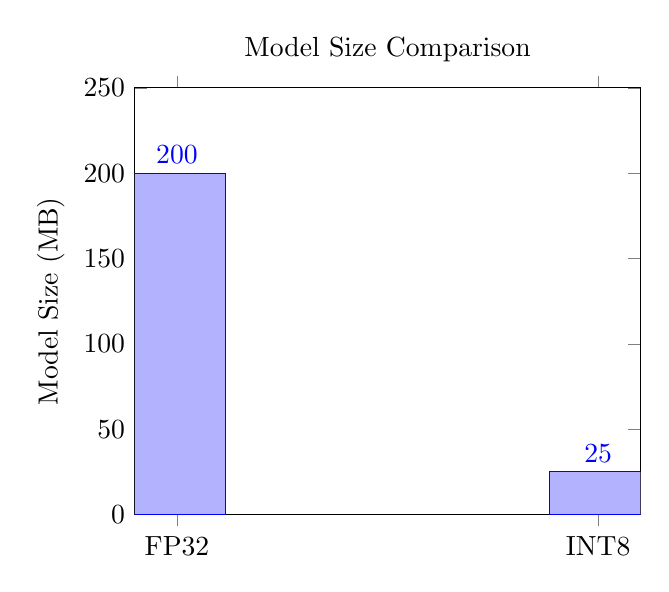
\begin{tikzpicture}
\begin{axis}[
    ybar,
    bar width=35pt,
    ylabel={Model Size (MB)},
    symbolic x coords={FP32, INT8},
    xtick=data,
    ymin=0, ymax=250,
    nodes near coords,
    nodes near coords align={vertical},
    width=8cm, height=7cm,
    title={Model Size Comparison},
    fill=blue!40
]
\addplot coordinates {(FP32, 200) (INT8, 25)};
\end{axis}
\end{tikzpicture}
\caption{FP32 vs INT8 Model Size}
\label{fig:model_size}
\end{figure}

\begin{figure}[H]
\centering
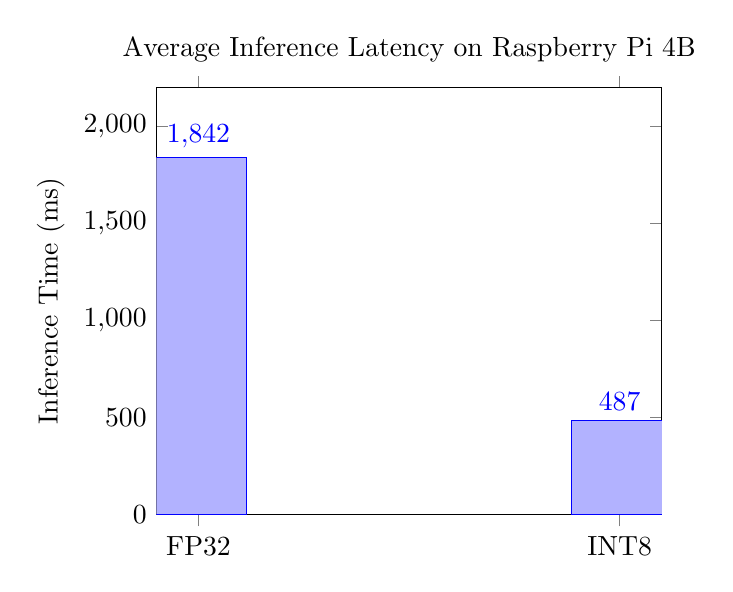
\begin{tikzpicture}
\begin{axis}[
    ybar,
    bar width=35pt,
    ylabel={Inference Time (ms)},
    symbolic x coords={FP32, INT8},
    xtick=data,
    ymin=0, ymax=2200,
    nodes near coords,
    nodes near coords align={vertical},
    width=8cm, height=7cm,
    title={Average Inference Latency on Raspberry Pi 4B},
    fill=red!40
]
\addplot coordinates {(FP32, 1842) (INT8, 487)};
\end{axis}
\end{tikzpicture}
\caption{FP32 vs INT8 Inference Latency}
\label{fig:inference_speed}
\end{figure}

\section{WebSocket Server Implementation}
\subsection{Server Architecture}
The edge server uses Python's \texttt{asyncio} event loop with the \texttt{websockets} library. Each client connection spawns a coroutine that processes frames sequentially:

\begin{algorithm}[H]
\caption{WebSocket Server Main Loop}
\begin{algorithmic}[1]
\Function{Main}{}
    \State Load ONNX model into InferenceSession
    \State Initialize EasyOCR reader
    \State Initialize SQLite connection
    \State Start WebSocket server on port 8765
    \State Run asyncio event loop forever
\EndFunction
\\
\Function{HandleConnection}{$websocket$}
    \For{each $message$ in $websocket$}
        \State $image \gets$ cv2.imdecode($message$)
        \State $input \gets$ preprocess($image$, 640, 640)
        \State $outputs \gets$ session.run(None, \{``images'': $input$\})
        \State $boxes, scores \gets$ postprocess($outputs$)
        \State $response \gets$ \{\}
        \For{each ($box$, $score$) in ($boxes$, $scores$)}
            \State $crop \gets$ image[$box.y1$:$box.y2$, $box.x1$:$box.x2$]
            \State $texts \gets$ reader.readtext($crop$)
            \State $plate \gets$ clean\_and\_validate($texts$)
            \If{$plate$ is valid}
                \State $record \gets$ db.lookup($plate$)
                \If{$record$ exists}
                    \State $response \gets$ verification\_payload($record$)
                \EndIf
            \EndIf
        \EndFor
        \State Send JSON($response$) to $websocket$
    \EndFor
\EndFunction
\end{algorithmic}
\end{algorithm}

\section{iOS Client Implementation}
\subsection{Camera Capture Pipeline}
The iOS app uses AVFoundation to capture camera frames. The pipeline is:
\begin{enumerate}
    \item \texttt{AVCaptureSession} configured with \texttt{.hd1280x720} preset.
    \item \texttt{AVCaptureVideoDataOutput} delivers \texttt{CMSampleBuffer} frames.
    \item Each frame is converted to JPEG via \texttt{UIImage.jpegData(compressionQuality: 0.6)}.
    \item JPEG data sent as binary WebSocket message.
    \item Server response parsed and detection overlay updated.
\end{enumerate}

\subsection{Detection Overlay Rendering}
The iOS app renders bounding boxes using a custom SwiftUI overlay:
\begin{itemize}
    \item Green rectangles indicate detected plates.
    \item OCR text is displayed above each bounding box.
    \item Coordinates are scaled from the model's 640$\times$640 space to the camera preview dimensions.
    \item Overlays update at the server's response rate (2+ FPS).
\end{itemize}

\section{Implementation -- Models Used}
\begin{enumerate}
    \item \textbf{YOLOv11:} Real-time license plate detection. Quantized FP32 $\to$ INT8. ONNX Runtime deployment.
    \item \textbf{EasyOCR:} CRNN-based text extraction from cropped plate regions.
    \item \textbf{Custom ONNX Patcher:} INT8 $\to$ UINT8 weight conversion for ARM compatibility.
\end{enumerate}

\section{Development Tools}
\begin{enumerate}
    \item \textbf{Git \& GitHub:} Version control and collaboration.
    \item \textbf{Google Colab:} GPU environment for model training and quantization.
    \item \textbf{Xcode 15:} iOS application development.
    \item \textbf{Visual Studio Code:} Python server development.
    \item \textbf{ONNX Runtime:} Quantized model execution on ARM.
    \item \textbf{Python \& Jupyter Notebook:} Prototyping and experimentation.
\end{enumerate}
